% \documentclass[journal]{vgtc}                % final (journal style)
%\documentclass[review,journal]{vgtc}         % review (journal style)
%\documentclass[widereview]{vgtc}             % wide-spaced review
%\documentclass[preprint,journal]{vgtc}       % preprint (journal style)
%\documentclass[electronic,journal]{vgtc}     % electronic version, journal

%% Uncomment one of the lines above depending on where your paper is
%% in the conference process. ``review'' and ``widereview'' are for review
%% submission, ``preprint'' is for pre-publication, and the final version
%% doesn't use a specific qualifier. Further, ``electronic'' includes
%% hyperreferences for more convenient online viewing.

%% Please use one of the ``review'' options in combination with the
%% assigned online id (see below) ONLY if your paper uses a double blind
%% review process. Some conferences, like IEEE Vis and InfoVis, have NOT
%% in the past.

%% Please note that the use of figures other than the optional teaser is not permitted on the first page
%% of the journal version.  Figures should begin on the second page and be
%% in CMYK or Grey scale format, otherwise, colour shifting may occur
%% during the printing process.  Papers submitted with figures other than the optional teaser on the
%% first page will be refused.

%% These three lines bring in essential packages: ``mathptmx'' for Type 1
%% typefaces, ``graphicx'' for inclusion of EPS figures. and ``times''
%% for proper handling of the times font family.

% \usepackage{mathptmx}
% \usepackage{graphicx}
% \usepackage{times}
% \usepackage{balance}  % to better equalize the last page
% %\usepackage[T1]{fontenc}
% \usepackage{txfonts}
% % \usepackage[pdftex]{hyperref}
% % \usepackage{url}      % llt: nicely formatted URLs
% \usepackage[usenames,dvipsnames]{xcolor}
% \usepackage{color}
% \usepackage{xspace}
% % \usepackage{amsmath}
% \usepackage{csquotes}

% \newcommand{\todo}[1]{\textcolor{blue}{[TODO] #1}\PackageWarning{template}{[TODO] #1}}

% % \newcommand{\comment}[1]{#1}
% \newcommand{\comment}[1]{}

% \newcommand{\joschi}[1]{\textcolor{NavyBlue}{[#1]}}
% \newcommand{\enrico}[1]{\textcolor{RedOrange}{[#1]}}
% \newcommand{\adam}[1]{\textcolor{RoyalPurple}{[#1]}}
% \newcommand{\eg}{\emph{e.g.}\xspace}
% \newcommand{\ie}{\emph{i.e.}\xspace}
% \newcommand{\etal}{\emph{et~al.}\xspace}
% \newcommand{\etc}{\emph{etc.}\xspace}

% % \newcommand{\ainfo}[1]{\phantom{#1}}
% \newcommand{\ainfo}[1]{#1}

%% We encourage the use of mathptmx for consistent usage of times font
%% throughout the proceedings. However, if you encounter conflicts
%% with other math-related packages, you may want to disable it.

%% This turns references into clickable hyperlinks.
% \usepackage[bookmarks,backref,linkcolor=black]{hyperref} %,colorlinks
% \hypersetup{
%   pdfauthor = {},
%   pdftitle = {},
%   pdfsubject = {},
%   pdfkeywords = {},
%   colorlinks=true,
%   linkcolor= black,
%   citecolor= black,
%   pageanchor=true,
%   urlcolor = black,
%   plainpages = false,
%   linktocpage
% }

%% If you are submitting a paper to a conference for review with a double
%% blind reviewing process, please replace the value ``0'' below with your
%% OnlineID. Otherwise, you may safely leave it at ``0''.
% \onlineid{0}

%% declare the category of your paper, only shown in review mode
% \vgtccategory{Research}

%% allow for this line if you want the electronic option to work properly
% \vgtcinsertpkg

%% In preprint mode you may define your own headline.
%\preprinttext{To appear in an IEEE VGTC sponsored conference.}

%% Paper title.

% [JK] the ~ are to force the line break at the right position
% do not remove!
% \chapter{Explain~It~All:~A~User~Study~on~the~Effect~of Aggregating~Explanations~for~Diagnosing~Machine~Learning~Models}
% \title{Using aggregated instance level explanations to detect hidden biases in your data}

%% This is how authors are specified in the journal style

%% indicate IEEE Member or Student Member in form indicated below
% \author{
% Anonymous Submission \#1264 \\
% Josua Krause,
% Adam Perer,
% Enrico Bertini
% }
% \authorfooter{
%% insert punctuation at end of each item
%  \item
%   \ainfo{Josua Krause is with NYU (josua.krause@nyu.edu)}
%  \item
%   \ainfo{Adam Perer is with IBM Research (adam.perer@us.ibm.com)}
%  \item
%   \ainfo{Enrico Bertini is with NYU (enrico.bertini@nyu.edu)}
% }

%other entries to be set up for journal
% \shortauthortitle{Krause \MakeLowercase{\etal}: Navigate instance level explanations through aggregation}

%% Abstract section.
\begin{quote}\textit{
Recently, there is growing consensus of the critical need to have better techniques to explain machine learning models.  However, many of the popular techniques are instance-level explanations, which explain the model from the point of view of a single data point.  While local explanations may be misleading, they are also not human-scale, as it is impossible for users to read explanations for how the model behaves on all of their data points.  Our paper explores the effectiveness of providing instance-level explanations in aggregate, by demonstrating that such aggregated explanations have a significant impact on users' ability to detect biases in data.
This is achieved by comparing meaningful subsets, such as differences between ground truth labels, predicted labels, and correct and incorrect predictions, which provide necessary navigation to explain machine learning models.
}
\end{quote}

\begin{quote}
\textit{Josua Krause, Adam Perer, Enrico Bertini}
\end{quote}

\begin{contributions}{Foo}
\item \todo{TODO}
\end{contributions}

% Recently, instance-level explanations have become a popular tool to inspect machine learning models and build a mental model of their behavior.
% However, those explanations are typically presented to the user one instance at a time.
% In order to make informed decisions about an analyzed machine learning model a data scientist needs to review examples in order to gain a holistic view of the model.
% This might be possible with relatively small data sets but becomes in-feasible when a user has to look at ${\sim}1,000$ instances.
% We explore how aggregating and providing navigation for those instance-level explanations can be an effective way of trusting model decisions and demonstrate its ability to help detect data sets with inherent biases using a controlled study on Amazon Mechanical Turk.
% For this, we generated data sets with known biases and let participants compare them to their unbiased counterparts.
% Enrico's title:
% "A User Study on the Effect of Visual Aggregation and Feature Weighting on Interpretation of Machine Learning Models"
% Adam's attempt:
% Explaining Predictions in Aggregate: A User Study on the Effect of Explanations for Interpreting Machine Learning Models
 % end of abstract

%% Keywords that describe your work. Will show as 'Index Terms' in journal
%% please capitalize first letter and insert punctuation after last keyword
% \keywords{Machine Learning, Classification, Interpretation, Visual Analytics, Study, Instance Level Explanations.}

%% ACM Computing Classification System (CCS). 
%% See <http://www.acm.org/class/1998/> for details.
%% The ``\CCScat'' command takes four arguments.

% \CCScatlist{ % not used in journal version
%  \CCScat{K.6.1}{Management of Computing and Information Systems}%
% {Project and People Management}{Life Cycle};
%  \CCScat{K.7.m}{The Computing Profession}{Miscellaneous}{Ethics}
% }

%% Uncomment below to include a teaser figure.
\begin{figure}
 \centering
 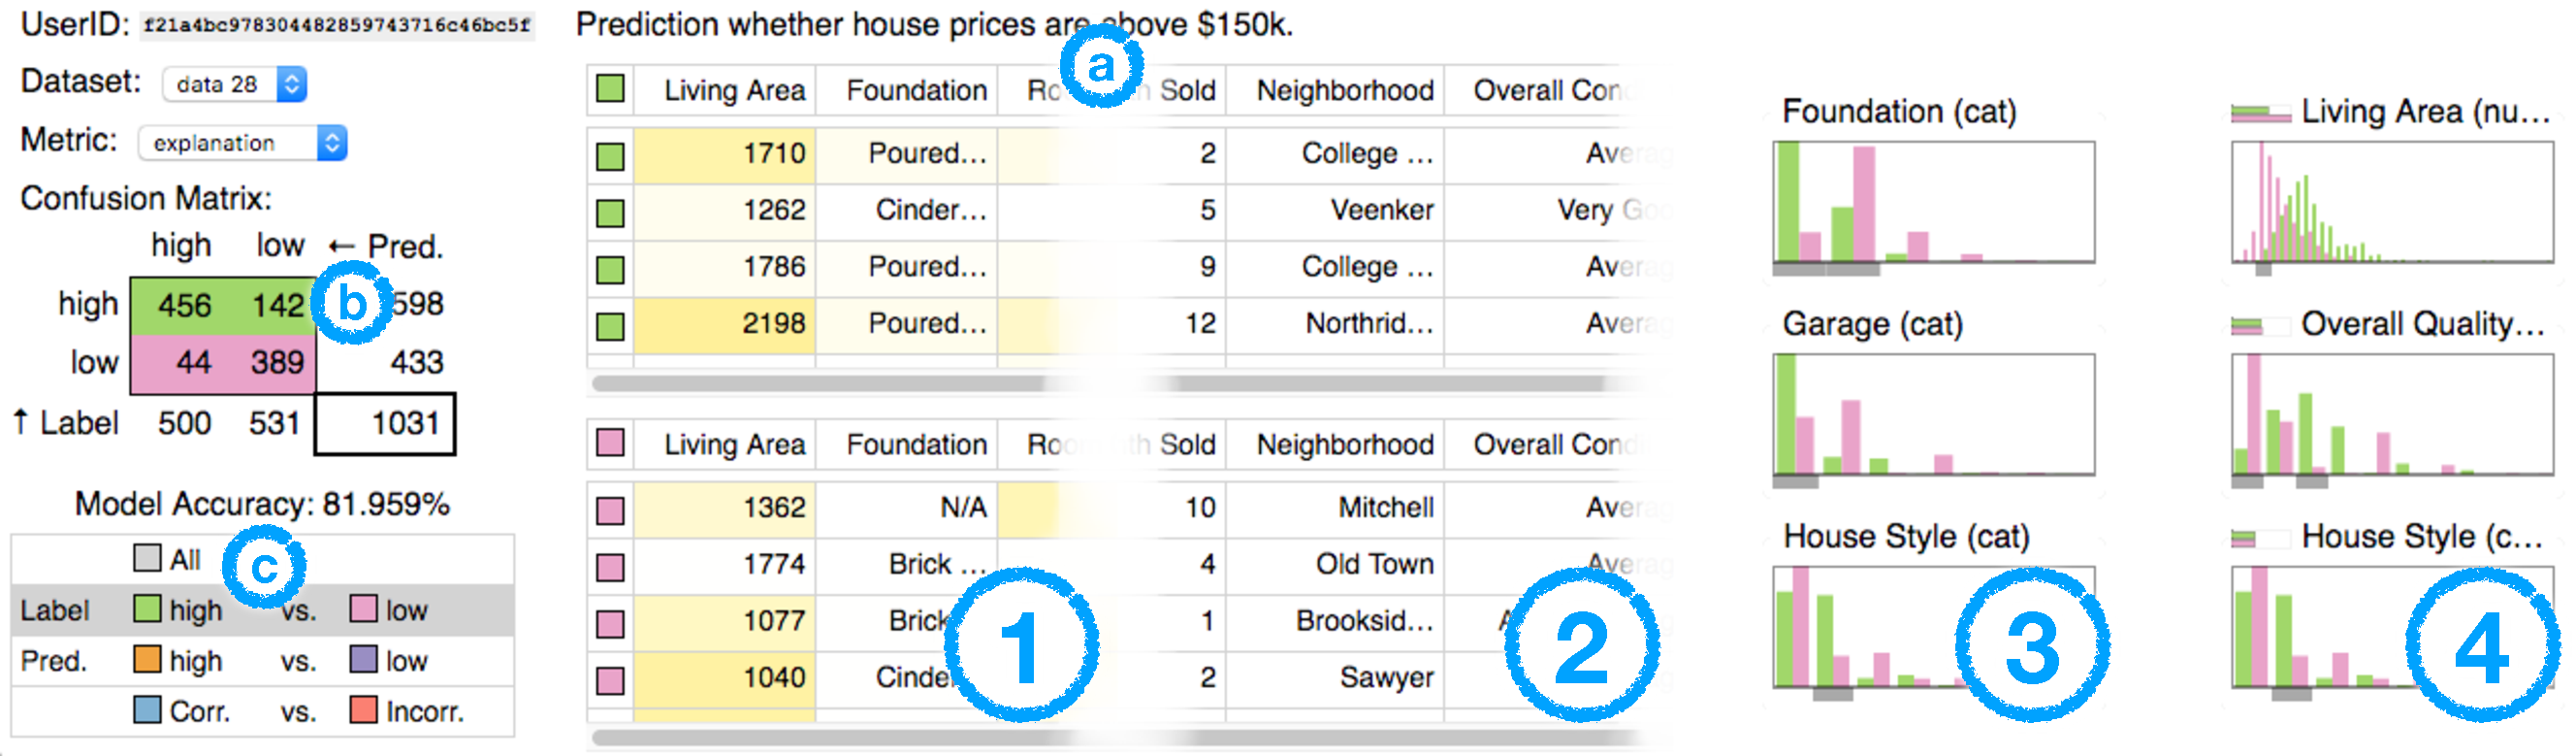
\includegraphics[width=0.8\textwidth]{aggexplain/teaser.pdf}
 \caption[Showing the four study conditions.]{
Showing the four conditions of our study: (1) instance-level explanations; (2) only instances; (3) only aggregated features; (4) aggregated features with explanations.
On the left and the top are consistent parts of the user interface showing: (a) the problem description; (b) the confusion matrix; (c) the subset selector.
%\adam{This teaser is a bit confusing. Would it be better to just have the complete UI here and this figure later.}
% I keep it for now
 }
 \label{figs:teaser}
\end{figure}

%% Uncomment below to disable the manuscript note
%\renewcommand{\manuscriptnotetxt}{}

%% Copyright space is enabled by default as required by guidelines.
%% It is disabled by the 'review' option or via the following command:
% \nocopyrightspace

%%%%%%%%%%%%%%%%%%%%%%%%%%%%%%%%%%%%%%%%%%%%%%%%%%%%%%%%%%%%%%%%
%%%%%%%%%%%%%%%%%%%%%% START OF THE PAPER %%%%%%%%%%%%%%%%%%%%%%
%%%%%%%%%%%%%%%%%%%%%%%%%%%%%%%%%%%%%%%%%%%%%%%%%%%%%%%%%%%%%%%%%

% \begin{document}

%% The ``\maketitle'' command must be the first command after the
%% ``\begin{document}'' command. It prepares and prints the title block.

%% the only exception to this rule is the \firstsection command
\section{Introduction}

% \maketitle

%% \section{Introduction} %for journal use above \firstsection{..} instead

As data continues to increase in complexity and scale, data scientists are increasingly turning to machine learning to automatically make decisions.  However, when these decisions are applied to high-stakes domains such as medicine, law enforcement, and financial lending, it is critical for humans to understand the basis for these decisions.

% We analyze the effect of providing aggregation and navigation for instance level explanations on trust and the ability to generate diagnostic insights of predictive models.

Predictive modeling is an area of supervised machine learning which aims to predict outcomes from data.
Such models are trained on examples with a known ground truth.  In order to verify that a model generalizes well to unseen data, a hold-out data set with known ground truth is typically used to test the model after training.
This allows to detect problems with the model, such as over-fitting on the training data, \ie, the model learned a phenomenon that is only present in the training data, by measuring the gap in the accuracy between the training and the testing data.
However, sometimes a bias in the collected data affects both the training and the test data which makes it impossible to detect through accuracy alone.
A human understanding of the underlying data is needed.

For example, Caruana~\etal\cite{Caruana:2015:IMH:2783258.2788613} built an interpretable machine learning model to analyze mortality risk in patients diagnosed with Pneumonia.
After analyzing the model's behavior, Caruana~\etal detected that patients that additionally suffered from Asthma had a significantly lower mortality risk, according to the \emph{model} and supported by the data.
However, this finding goes against current medical knowledge, as the combination of Pneumonia and Asthma are associated with a significantly increased mortality risk.
In fact, the data was biased because these high-risk patients with Asthma were given special attention during their hospital visits which contributed to their lower mortality.  The presence of Asthma was not responsible for their improvement in health, but rather a systematic bias. 

\begin{figure}[t]
 \centering
 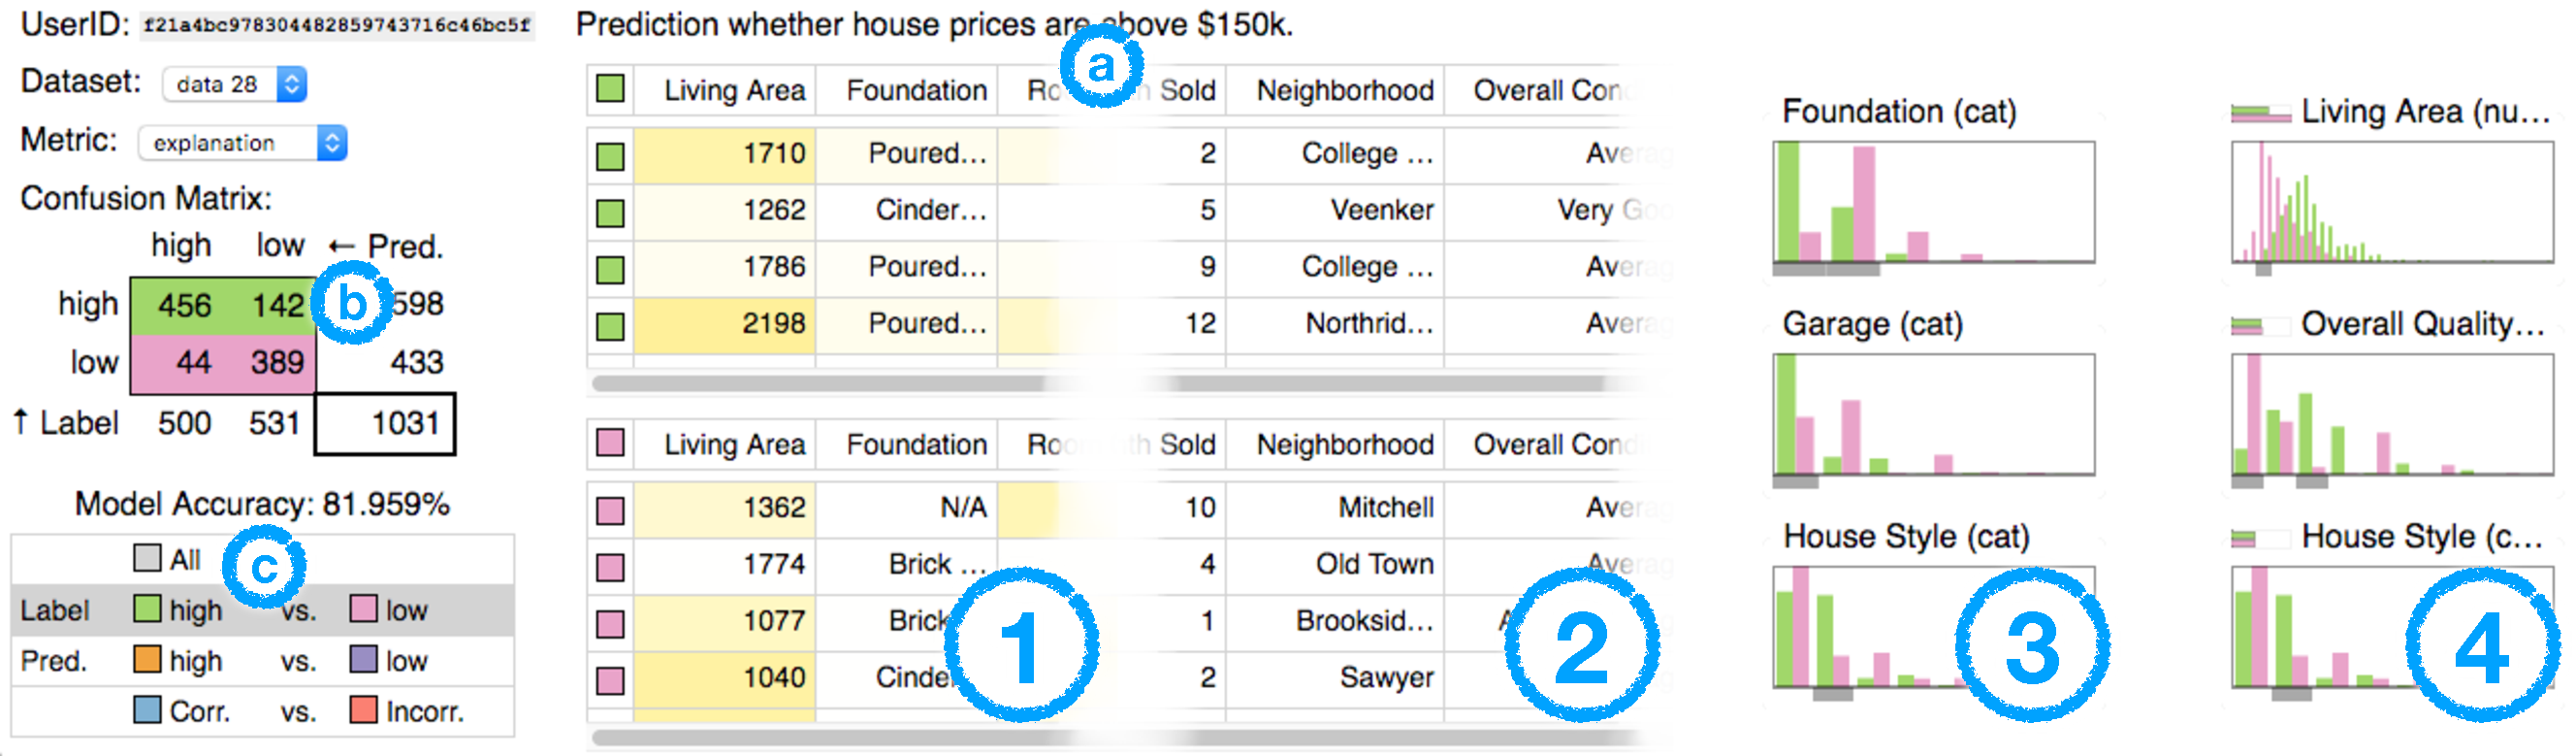
\includegraphics[width=\linewidth]{aggexplain/teaser.pdf}
 \caption[Showing the four study conditions.]{
Showing the four conditions of our study: (1) instance-level explanations; (2) only instances; (3) only aggregated features; (4) aggregated features with explanations.
On the left and the top are consistent parts of the user interface showing: (a) the problem description; (b) the confusion matrix; (c) the subset selector.
%\adam{This teaser is a bit confusing. Would it be better to just have the complete UI here and this figure later.}
% I keep it for now
 }
 \label{figs:teaser}
\end{figure}

Using the interpretable model and human expert knowledge, it was possible to detect this systematic bias in the data before deploying the model.
However, using interpretable machine learning algorithms typically penalizes their capacity, thus lowering the potential accuracy of the model \cite{Caruana:2015:IMH:2783258.2788613} or is only superficially more interpretable by being interpretable on a small scale but not for more complex tasks (\cite{lipton2016mythos,2016arXiv160605685K}).
As a way to interpret the behavior of machine learning models \emph{independently} from the used algorithm, black-box and more precisely, instance-level explanations recently became popular \cite{Martens:2014:EDD:2600518.2600523,DBLP:journals/corr/RibeiroSG16,prospector}.

However, such explanations are commonly reviewed by experts one-at-a-time.
This task becomes infeasible when dealing with thousands or more instances, also typical of real-world datasets.
To that extent, we propose a visual way of reviewing instance level explanations with the help of aggregation in combination with navigation.
This is implemented through the comparison of subsets of the test data under different conditions.

\begin{figure}[t]
\centering
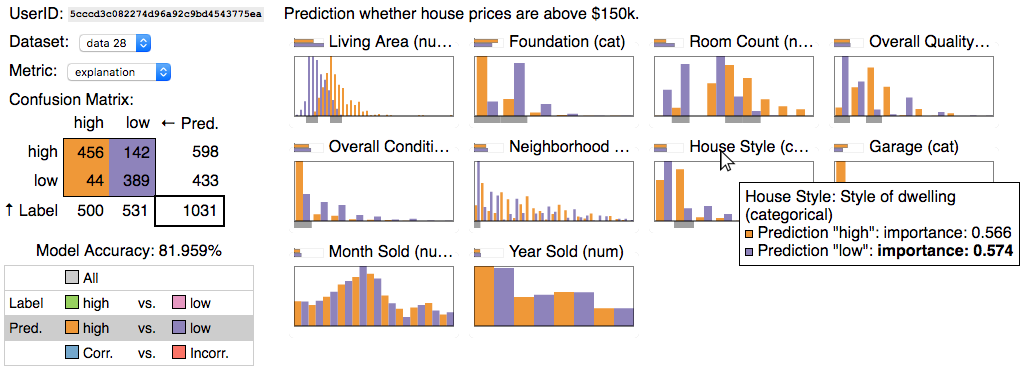
\includegraphics[width=\linewidth]{aggexplain/full_histogram}
\caption[The full interface illustrating the aggregated histogram view.]{
The full interface illustrating the aggregated histogram view.
The user is comparing the model's prediction of ``high'' house prices (orange) to the prediction of ``low'' prices (purple).
The user hovers over the feature ``House Style'' revealing a more detailed description, whether the feature is categorical or numeric, and the importance / feature weight for each of the subsets.
}
\label{figs:full_hist_view}
\end{figure}

We conducted a study comparing aggregated instance-level explanations to their individual counterparts.
Under both conditions different subsets of the test data could be compared by participants.
By providing models with both biased and unbiased data we were able to measure the trust of participants in the decisions made by the models and their ability to detect flaws in the underlying data for both methods.

Concretely, our contributions include a method for effectively comparing subset of a data set using histograms; using this method, a way to effectively aggregate instance-level explanations; and a study showing that this aggregation overcomes the potential harmfulness of instance-level explanations.
% \begin{itemize} %[leftmargin=*,noitemsep,nolistsep]
% \item \textbf{Design:} Techniques for Comparison,Y,Z. 
% \item \textbf{User Study:} Shows A,B,C
% \end{itemize}
% \todo{Fill in bulletpoints}

Following, we will first discuss related work in Section~\ref{sec:relatedwork} and then motivate the circumstances of our study further in Section~\ref{sec:motivation}.
We will propose our design for aggregating and comparing subsets of instance-level explanations in Section~\ref{sec:design}.
Afterwards we will describe the experimental setup in Section~\ref{sec:setup}.
The results of the study are provided in Section~\ref{sec:results} and their implications are discussed in Section~\ref{sec:ag_discussion}.
We then conclude in Section~\ref{sec:conclusion} and discuss future work.

\section{Related Work}
\label{sec:relatedwork}

We broadly divide related work into two parts.
Studies focusing on the effectiveness of instance-level explanations and attempts in detecting bias, using visual analytics, in data provided to machine learning models.

%\adam{This needs to be organized in some way, rather than just a list of work. -- low priority right now}

\subsection{Effectiveness of instance-level explanations}
When introducing their algorithm, LIME (Ribeiro~\etal~\cite{DBLP:journals/corr/RibeiroSG16, anchors:aaai18,2016arXiv161105817T}), the authors conducted experiments to show the effectiveness of their method.
However, instance-level explanations were only inspected individually and not in aggregate form.

Kulesza~\etal~\cite{Kulesza:2015:PED:2678025.2701399} introduced explanatory debugging.
Users are presented individual decisions, made by the model, in a list.
Those can then can be used to ``personalize'' the model and improve its statistical performance by finding and giving feedback on incorrect decisions.

%https://csjzhou.github.io/homepage/papers/INTERACT2017_Effects_Trust.pdf
Zhou~\etal~\cite{Zhou:2017:EUC:3176444.3176447} analyzes how uncertainty and cognitive load affects trust in a machine learning model.
Here models are compared that predict the risk of pipe failure in a sewer systems according to several features.
In addition to the expected failure rate according to model, the length of the observed part of the pipes is shown to the user aggregated over all instances.
The study found that showing the uncertainty of the model significantly decreased the trust of participants.
Additionally, adding cognitive load in terms of limited decision time trust in the model decreased significantly as well.

Narayanan~\etal~\cite{2018arXiv180200682N} explored how humans understand explanations from a machine learning model.
Explanations for individual instances, in the form of simple rules, were presented and participants were asked to determine the predicted outcome of the underlying model.
The study found that greater complexity, more rules and more variables, resulted in a higher response time and decreased accuracy.

Note, that the works presented so far always assume that errors stem from the shortcomings of the model and not from incorrect or biased data.

Stumpf~\etal~\cite{harmful} found that under some circumstances, explanations can be harmful to the end user, by invoking false confidence.
This is on one hand due to the user extrapolating from few instance-level explanations, making their mental model seem correct.
And, on the other hand, trust in the machine learning model \emph{overrides} their initial intuition: ``I guess this thing knows more than me. The system knows more than me. I'll accept [the diagnosis]''.
We could confirm both of those findings in our experiments.

\subsection{Detecting biases using visual analytics methods}
Hohman~\etal~\cite{2018arXiv180106889H} identifies detecting biased data as one of their five use cases for visual analytics for machine learning.
However, their examples focus on work that only looks at the data without the help of machine learning models~\cite{facets} or simple models where humans adjust the thresholds of the model manually~\cite{wattenberg}.

Chang~\etal~\cite{revolt-collaborative-crowdsourcing-labeling-machine-learning-datasets} uses crowd-sourcing to label data and ensure its integrity.
However, this approach does not work if domain expertise in the field is required to label data correctly.

Simard~\etal~\cite{DBLP:journals/corr/SimardACPGMRSVW17} introduces Machine Teaching.
This paradigm uses an already labeled data set for training a machine learning model.
It then presents predicted instances to a domain expert who then can either, fix an incorrect label, manipulate features, change constrains, or post-pone a decision if the instance is ambiguous.
This way an expert can ensure that the final model is correct and remove biases.
However, finding biases is not scalable as the experts has to go through many examples and might miss problems, especially if the performance of the model increases but the underlying data is incorrect.

Krause~\etal~\cite{explainer} demonstrates, how aggregated instance-level explanations can be used to find biases in hospital data.
They used an instance-level algorithm optimized for sparse binary input data (Martens and Provost~\cite{Martens:2014:EDD:2600518.2600523}).
Through aggregation, filtering, and reordering, they found biases in their data used for predicting hospital admission that made it impossible for the machine learning model to correctly predict admission in some cases.
For example, the model knew about a CET or PET scan happening but was unaware of their results.
Thus, the model was unable to predict the diagnosis since the result of the scan directly influences the outcome.



% not worth it / not fitting
%https://www.propublica.org/article/machine-bias-risk-assessments-in-criminal-sentencing
%\cite{dasgupta2017familiarity}
%\cite{2017arXiv171100867K}
%Lei~\etal~\cite{DBLP:journals/corr/LeiBJ16}

\section{Motivation}
\label{sec:motivation}
% \adam{Right now, this is written as motivation for the study.  You may want to consider re-writing this as motivation for the need for aggregated explanations instead... and move the experiment-specific motivation to the experiment section.  This depends if you end up creating a new section for the Design contribution or not.}

Experiments for instance-level explanations typically focus on use cases where the explanation is presented to the user one instance at a time. This is helpful when monitoring the continuous performance of a machine learning model in production. However, it limits one's ability to gather a holistic view of a model's behavior (\ie, a global explanation). Looking at many instances is very time consuming and potentially ineffective. It is not clear whether people can build a coherent understanding of a model by looking at a series of instances: comparison between many instances overloads memory and does not leverage the data compression capabilities of aggregate representations.

The main goal of our study is therefore to explore the idea of aggregating data about many instances and their explanations and verify its effects on model comprehension. More precisely, we want to study the effect of aggregation on what we call ``semantic validation'': the ability of a human to validate the decisions of a model according to his or her knowledge of the domain.

For this purpose, somebody knowledgeable with the domain has to verify that the model and the data are consistent with their mental model and, if necessary, override information coming from statistical aggregates on accuracy. This is an important task, especially for models making critical decisions such as those employed in health care~\cite{Caruana:2015:IMH:2783258.2788613} and security.

A second goal of this study is to better understand how explanations contribute to semantic validation. Explanations typically provide, for each instance, a weight or score that conveys information about how important each feature is, for a given decision, and for a given instance. An important question therefore is to better understand what particular benefits, if any, explanations bring to human validation; whether this is conducted using an instance-level exploration strategy or a more compact aggregation. Our hypothesis is that explanations may bring value if they manage to direct the user's attention to instances and features where biases and mistakes reside.

In summary, our experiment aims at studying the effect of two main factors: \textit{aggregation level}, that is, instances vs. aggregations, and explanations, that is, whether feature weights are present or not.

% Instance-level explanations provide an effective way of focusing the attention of a user towards which features are important for a prediction. If a bias in a data set has a non-negligible effects on the semantic quality of the prediction, then this bias will show up in the set of important features.

% Note, that if the bias was in a feature that is never used by the model it would not affect the model's outcomes.

% However, a big disadvantage of instance-level explanations is that the instances have to be inspected individually. This might result in misleading conclusions as users have to extrapolate their general understanding of the machine learning model from the few instances they have inspected. Aggregating the explanations might be the key for improving semantic validation through instance-level explanations.

% Semantic validation works by detecting biases in the training and / or test data. Therefore, in order to study semantic validation we need ground truth data with known biases. We achieved that by manually creating a bias in an otherwise normal data set and using both to compare the detection of biases.

\section{Design Contribution}
\label{sec:design}
In order to effectively analyze machine learning behavior we allow users to compare subsets of the data set to each other.
These subsets are defined by different combinations of cells in the confusion matrix of the machine learning model.
We selected subsets that help understanding the behavior of the model:

\begin{description}
\item[All.] The full data set is shown and no comparison occurs. This is the initial view of the data.
\item[Ground truth.] By comparing rows of the confusion matrix to each other a user can explore the actual labels of the data.
\item[Predicted labels.] By comparing columns of the confusion matrix to each other a user can explore the predicted labels of the model.
\item[Correctness.] By comparing the diagonals of the confusion matrix to each other a user can explore when the model's prediction is correct or incorrect.
\end{description}

It is thinkable to allow more freedom in selecting subsets to, \eg, compare only errors of a certain predicted label, however, this would increase the complexity of the user interface and a user has to understand when to use each of those subsets in order to be effective.

\begin{figure}[t]
\centering
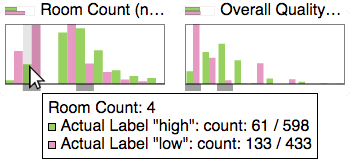
\includegraphics[width=0.7\linewidth]{aggexplain/histogram}
\caption[Comparing the distribution of values by ``Actual Label''.]{
Comparing the distribution of values by ``Actual Label'' (\ie, ground truth).
The height of the bars show the percentage of values within the respective subset (green for ``high'' outcomes and pink for ``low'' outcomes).
The average feature weight of each subset is shown next to the feature name.
This is only visible in the condition including explanations.
}
\label{figs:histogram}
\end{figure}

When aggregating instances, comparing subsets to each other is not trivial.
The na\"ive solution of showing the actual amount of instances with respect to the full data set disadvantages the smaller subset.
However, it is not as important to know the actual distribution, but rather where one subset has a significantly higher or lower concentration of instances compared to the other.
To this extend we propose a novel approach of scaling each subset separately with respect to their own magnitude (see Figure~\ref{figs:histogram}).
Note, that we then compare percentages of instances within the respective subsets.
We further indicate strong differences in the subsets by showing a gray bar at the bottom of the histogram.
We are not aware of any literature that uses or explored this way of comparing subsets with histograms and claim it as a design contribution.
We demonstrate the effectiveness of this design in Section~\ref{sec:results}.

\begin{figure}
\centering
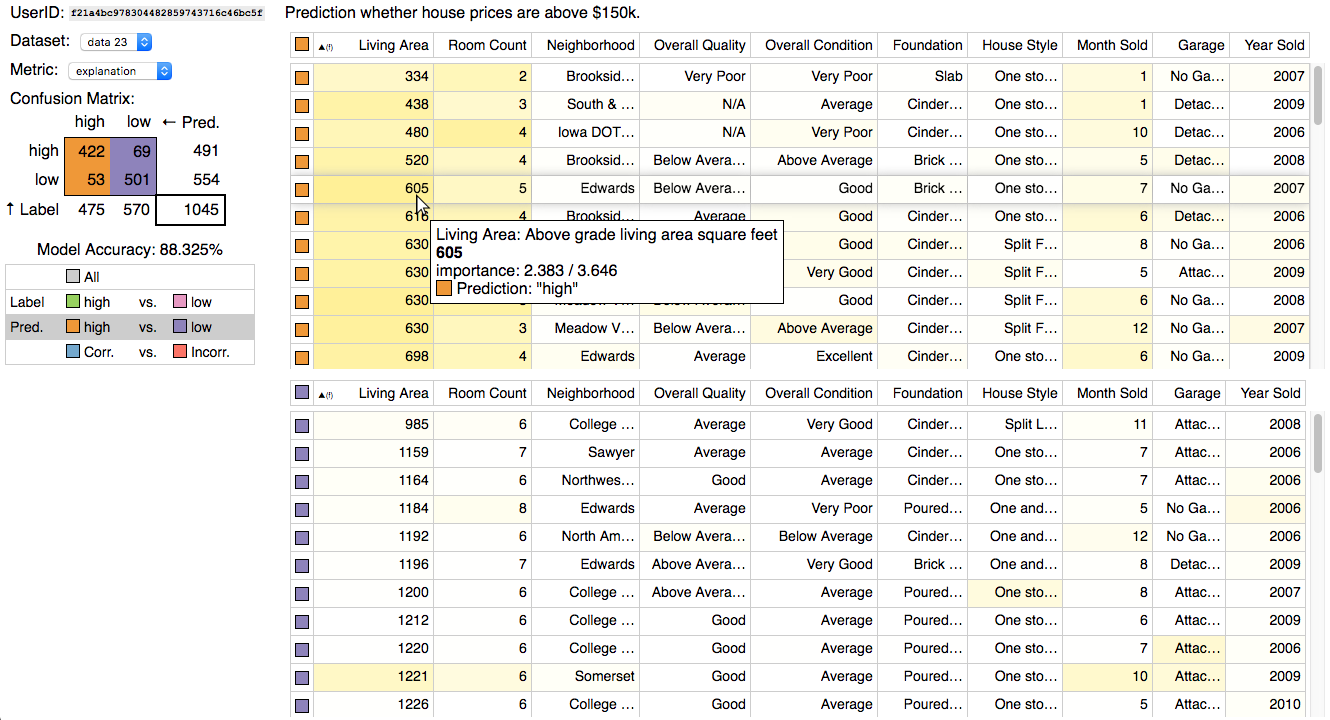
\includegraphics[width=\linewidth]{aggexplain/full_table_expl}
\caption[The full interface illustrating the table view.]{
The full interface illustrating the table view showing individual instances.
The user is comparing the model's prediction of ``high'' house prices (orange) to the prediction of ``low'' prices (purple).
The feature ``Living Area'' is ordered by ascending values and the user hovers over the cell with the value ``605''.
}
\label{figs:full_view}
\end{figure}

\section{Experimental Setup}
\label{sec:setup}
In order to see whether explanations are helpful in detecting biases of the training data we used the publicly available housing price data~\cite{housing} and created a version that has a bias that needs to be detected.
Originally a regression task, we converted the data set into a classification task predicting whether the house price is above \$150k (598 instances above; 433 instances below; 1031 instances in total).
We also reduced the number of features in the data set to 10 in order to make it possible to see all features at once in all conditions, without the need to scroll, so data otherwise hidden off-screen would not be a confounding effect.
The biased dataset needed to have a bias detectable in both the aggregated and instance-level version, thus we chose to manipulate the outcome of the biased data set to be dependent on the value of one feature (``Living Area'') with some random perturbations.
The biased outcome was chosen so that a \emph{larger} ``Living Area'' results in a \emph{lower} house price.
This relationship does not reflect reality (an increased ``Living Area'' generally results in a higher house price).
The bias is present to the same degree in both the training and the testing data.

Furthermore, by controlling the degree of randomness while creating the biased data set we controlled the accuracy of the prediction when training a machine learning model, such that the model using the biased data has a \emph{higher} accuracy than the model on the real data.
We trained Multi-Layer Perceptrons~\cite{mlp} on both data sets resulting in test accuracies of $81.96\%$ for the real data and $88.33\%$ for the biased data.

\subsection{User Interface Conditions}
For explaining the model behavior we computed the explanations using the LIME algorithm~\cite{DBLP:journals/corr/RibeiroSG16} on the test data.
LIME computes feature weights for each instance in the data.
A weight of zero indicates that the feature was not used in the prediction whereas a non-zero weight indicates that the feature was used.
A feature weight with larger magnitude indicates that the feature was more important to the prediction than a feature with a smaller magnitude of its weight.
However, in order to simplify the user interface and understanding, we computed the absolute value of the feature weights.
Thus, participants will only see if a feature has influence on the prediction, not whether this influence is towards a ``low'' or ``high'' house price prediction.
This additional information is not relevant for the given task and would make the user interface confusing.

For comparing instance-level and aggregated conditions we developed two user interfaces.
Both interfaces share two major components,
%\adam{I don't think you need to call out the short sentence as a separate  component: focus more on confusion matrix + systematic list}
%a short sentence describing the prediction task,
the confusion matrix of the current model alongside the model's accuracy and a list for selecting different subsets to compare to each other (see Figure~\ref{figs:teaser}).
Those subsets can be: comparing instances with different ground truth labels, instances with different predicted labels, instances with different correctness, or the full dataset in which case no comparison occurs.
How comparing subsets looks like is dependent on the which condition is used.
The selections use different colors to distinguish the subsets in order to prevent participants getting confused about which subset comparison is currently selected (we also indicate the selection in the list).
The colors are also used to highlight the confusion matrix cells corresponding to the current selection.
Note, that all selections always represent all instances in the data and no two instances from the same confusion matrix cell can appear in opposing subsets.

The design of the user interface lets users iterate through multiple useful slices of the data (such as getting an overview of the data or comparing different, meaningful, subsets to each other).
This design, inspired by SYF \cite{perer2008systematic}, provides users with a systematic guide to iterate through meaningful views while also supporting flexible diversions to pursue insights.
% \adam{Consider strongly making this a comparison discussion a section on its own (e.g. new Section 4, before Experiment, as its key for making it work.  Then, you could call this design out as a contribution in Intro.}

\subsubsection{Instance-level Condition}
The user interface for the instance-level condition is a table showing the values of each feature for each instance in its cells, as seen in Figure~\ref{figs:full_view}.
This is a change from how instance-level explanations are usually studied in the literature, where each instance is presented in isolation.
However, this way of showing instances is limiting as it becomes time consuming to inspect more instances so a participant would only see very few instances in total.

The columns of the table, representing features, are ordered by the average weight of this feature, if the condition includes explanations.
If the condition does not include explanations the columns are sorted alphabetically.
The cells of the table reflect the feature weight of the corresponding instance using a yellow color scale.
In addition to that, hovering over a cell with the mouse shows a tool-tip indicating the actual feature weight number and the full value of the cell and the full feature name in case those values got abbreviated due to cell size restrictions.

Columns can be sorted by clicking on the table header.
This cycles through sorting the feature values by ascending and descending value.
If explanations are available, the feature can also be sorted by ascending and descending feature weights.

For comparing different subsets of the data we show two aligned tables.
The colors representing the different subsets are shown on the far left side of the table.

\subsubsection{Aggregated Condition}
The user interface for the aggregated condition represents the distribution of feature values as histograms.
Feature names are shown above the histogram and the histograms are arranged left to right row-wise and top to bottom.
For the condition with explanations available, a small bar chart next to the feature name indicates the average weight of this feature.
In this condition, the histograms are ordered by descending magnitude of average feature weights.
The averages are computed for each subset separately.
The order is, more specifically, based on the average of the subsets' average weights, which allows features to appear first that are only important under certain conditions.
If no explanations are provided, the order is alphabetically.

Hovering over a histogram with the mouse reveals tool-tips showing the actual instance count of the hovered histogram segment, as well as, the full feature name and the feature weight number.
For categorical features the bars of the histograms are slimmer so that distinct values are more easily separable.
Additionally, the order of the values indicate their quantity in the data set with the most common categorical value first on the left.

When comparing different subsets of the data, as seen in Figure~\ref{figs:good_vs_bad}, bars of each color are shown next to each other in the histogram.
The height of the bars are scaled by their relative proportion \emph{within} each subset.
This means the height indicates the percentage of instances in the respective subset.
The vertical scale ranges to the highest percentage across both subsets.
This allows for seeing where one subset is more concentrated than the other independent of the total size of each subset.
In order to indicate big differences in the distribution we show a gray rectangle at the bottom of the histogram if one subset is strongly more concentrated at this value range than the other (see Figure~\ref{figs:histogram}).

\begin{figure}[t]
\centering
\raisebox{-0.5\height}{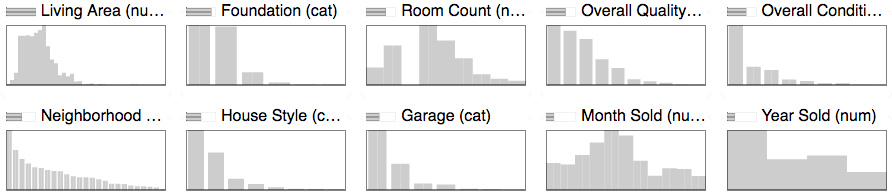
\includegraphics[width=0.4\linewidth]{aggexplain/h_all}}
\raisebox{-0.2\height}{
\parbox{0.16\linewidth}{
\centering
\tiny{\textsf{$\leftarrow$ Unbiased data set}}\\
\tiny{\textsf{Biased data set $\rightarrow$}}\\
\tiny{\textsf{Compared subset:}}\\

\includegraphics[height=0.75em]{aggexplain/legend_all}
}
}
\raisebox{-0.5\height}{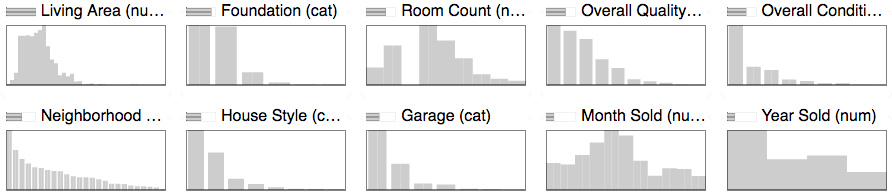
\includegraphics[width=0.4\linewidth]{aggexplain/h_all}}
~\\
\noindent\rule{\linewidth}{0.4pt}
~\\
\raisebox{-0.5\height}{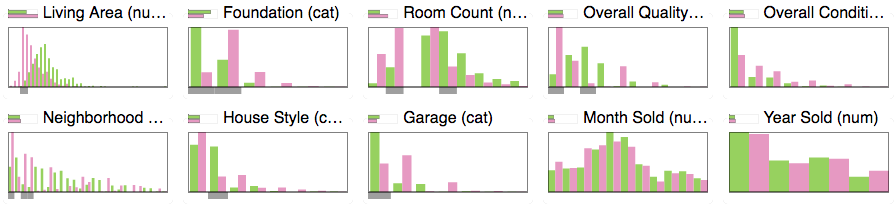
\includegraphics[width=0.4\linewidth]{aggexplain/h_label_ok}}
\raisebox{-0.2\height}{
\parbox{0.16\linewidth}{
\centering
\tiny{\textsf{$\leftarrow$ Unbiased data set}}\\
\tiny{\textsf{Biased data set $\rightarrow$}}\\
\tiny{\textsf{Compared subset:}}\\
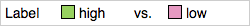
\includegraphics[height=0.75em]{aggexplain/legend_label}
}
}
\raisebox{-0.5\height}{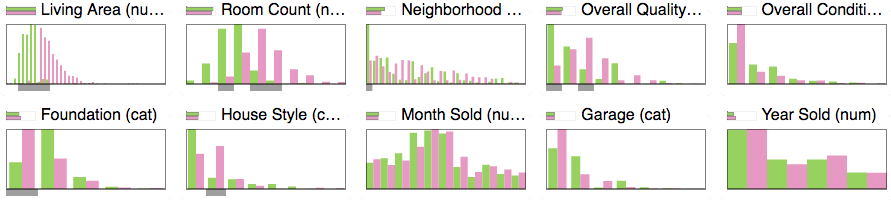
\includegraphics[width=0.4\linewidth]{aggexplain/h_label_bad}}
~\\
\noindent\rule{\linewidth}{0.4pt}
~\\
\raisebox{-0.5\height}{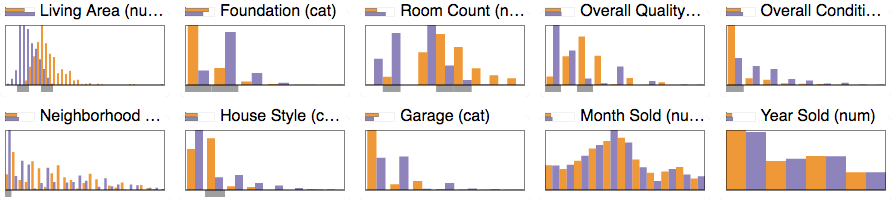
\includegraphics[width=0.4\linewidth]{aggexplain/h_pred_ok}}
\raisebox{-0.2\height}{
\parbox{0.16\linewidth}{
\centering
\tiny{\textsf{$\leftarrow$ Unbiased data set}}\\
\tiny{\textsf{Biased data set $\rightarrow$}}\\
\tiny{\textsf{Compared subset:}}\\

\includegraphics[height=0.75em]{aggexplain/legend_pred}
}
}
\raisebox{-0.5\height}{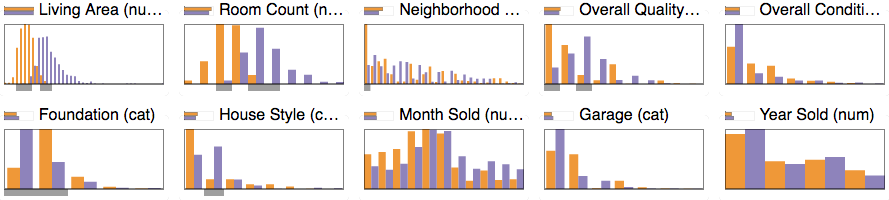
\includegraphics[width=0.4\linewidth]{aggexplain/h_pred_bad}}
~\\
\noindent\rule{\linewidth}{0.4pt}
~\\
\raisebox{-0.5\height}{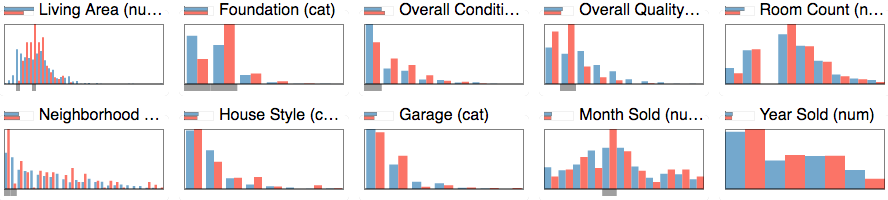
\includegraphics[width=0.4\linewidth]{aggexplain/h_correct_ok}}
\raisebox{-0.2\height}{
\parbox{0.16\linewidth}{
\centering
\tiny{\textsf{$\leftarrow$ Unbiased data set}}\\
\tiny{\textsf{Biased data set $\rightarrow$}}\\
\tiny{\textsf{Compared subset:}}\\

\includegraphics[height=0.75em]{aggexplain/legend_correct}
}
}
\raisebox{-0.5\height}{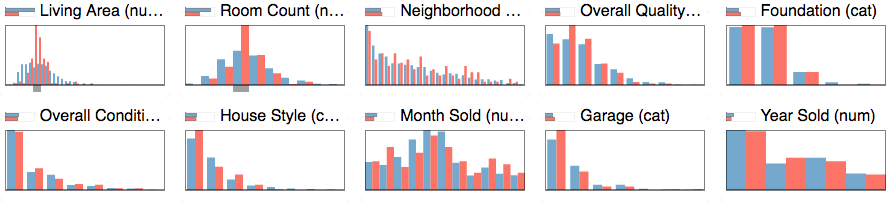
\includegraphics[width=0.4\linewidth]{aggexplain/h_correct_bad}}
\caption[Comparison of different subset selections on both models.]{
Comparison of different subset selections on both the unbiased model (left side) and the biased model (right side).
Features are sorted per segment by most important at the top-left, row-wise to least important at the bottom-right.
Note, the feature ``Living Area'', in both the ``Label'' (\ie, ground truth) and ``Pred.'' (\ie, model prediction), has flipped outcomes for the biased model (right side).
Each subset has a different color palette to not confuse different selections with each other.
}
\label{figs:good_vs_bad}
\end{figure}

\subsection{Study Design}
We study four conditions which result from combining different representations with the inclusion or exclusion of explanations.
The different representations are:

\begin{itemize}
	\item
    A view of the model through individual instances.
    Instances are listed in a table.
    This is an extension of the approach of inspecting instances one-by-one.
    \item
    A view of the model through aggregated instances.
    Instances are aggregated in histograms for individual features.
\end{itemize}

In each of those conditions we compare the ability to detect biases in the data by comparing the unbiased data set to the data set with the manufactured bias.

We also explore the impact of those conditions on whether explanations and aggregation improve trust in the model's decisions.
Particularly, trust in the \emph{right} model.

\subsection{Tasks and Measurements}
In order to test conditions against each other we created a questionnaire.
After asking the participant about the knowledge of machine learning and basic terminology, we have a training section for participants to familiarize themselves with the interface.
First, an introductory video explains all components of the interface.
The video uses an example model from a different data set which is designed to predict whether a room is occupied or not based on predictions from various sensors~\cite{occupancy}.
Then, a series of questions about this example model are asked and the participant can and has to use the interface to answer them correctly.
The questions ask about the values of features under certain conditions, such as ``What is the model's prediction for high values of `$CO_2$?''', ``What is the lowest value of `Humidity' that predicts `occupied'?'', ``Are the predictions for low values of `Light' correct?''.
The questions are constructed in a way to be easily answerable under all conditions given an understanding of the user interface and basic principles of machine learning.
An incorrect answer leads back to the beginning of the section and the participant is given the chance to correct the mistake.
We did not use those questions to exclude any participant but rather for giving them an opportunity to get comfortable with the user interface.
Note, that it is not necessary for participants to have a deep knowledge in \emph{how} machine learning algorithms work, as long as, the basic principles of prediction, ground truth, or accuracy are clear.  This reflects that domain experts would often not necessarily be trained in \emph{developing} machine learning models but rather \emph{using} them.

As final question of this segment the participant has to detect, in a hypothetical, scenario that a prediction does not make \emph{sense} from a semantic standpoint, even though that prediction is \emph{correct} from the perspective of the model.
This question aims to prime the participants for the upcoming task and teaches that model correctness is not necessarily equivalent to semantic correctness.
After this, we ask some common sense questions about how house prices are supposed to correspond to certain features.
This ensures that participants have enough domain knowledge for the upcoming task.

In the main part of the study we present the participant with both housing data models one after the other and encourage them to explore the models with the end goal of determining which model can be trusted more.
The order of the data sets is random.
The participant then has to answer the following questions about each model:
``Do you think the predictions of the model make sense?'',
``How well does the model perform in terms of accuracy?'',
``How much do you trust the model?''
on a five-point Likert scale;
and explain the reasoning for their answers.
For each question we provide a more in-depth explanation with examples.

After inspecting both models, we ask the participants to state which model performs better in terms of accuracy, which model can be trusted more, and whether the model they trust more had the higher or lower accuracy, or no model can be trusted more than the other.
We ask participants to describe their reasoning and also state their confidence in their decision on a five-point Likert scale.

\subsection{Participants}
We ran all four conditions of the study on Prolific\footnote{\url{https://www.prolific.ac/}}, an online survey recruitment system.
Participants in online recruitment aim to increase their payout to effort ratio.
Thus, we took several measures to ensure high data quality.
Firstly, we only allowed participants with a high rating on the platform and an interest in computer science.
Secondly, we excluded all data from participants that had a suspiciously fast completion times (less than 10 minutes after watching the introductory video) which would not allow them to establish well thought out answers.
We also excluded participants with too little interaction with the interface, determined by the number of histograms or table cells they inspected and how often they changed the subset comparison selection.
As attention question we used the question ``Which model had the higher accuracy?'' to remove participants.
This question has an objective answer that had to be determined during the study as well.
By reading the full text answers we could exclude participants that had little understanding of machine learning or the assigned task, or were giving non-sense answers.
We retained 100 eligible participants divided evenly across the four conditions.
This represents less than $47\%$ of total participants, not counting participants that stopped the study before submitting.

\section{Results}
\label{sec:results}
Following, we will perform an exploratory analysis of our study results.

\begin{figure}
\centering
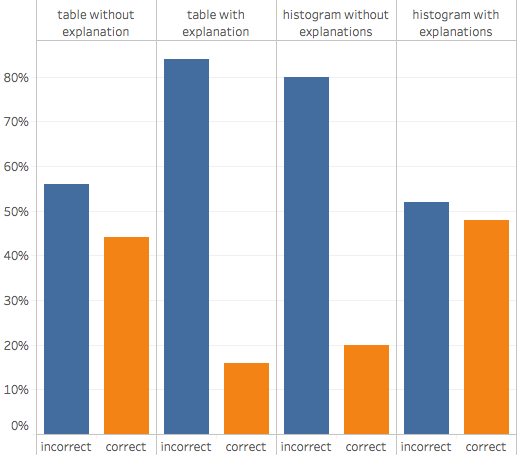
\includegraphics[width=0.5\linewidth]{aggexplain/correctness}
\caption{
Comparing whether participants correctly identified the bias in the data, determined from plain-text answers. Note, that adding explanations to the table view hurt performance, whereas adding explanations to the histogram view improved performance.
}
\label{figs:correctness}
\end{figure}

For reasons we will explore later, we used the plain-text answers of the participants to determine whether they correctly found the bias in the correct data set.
This is an unambiguous way, since participants were verbose about their findings (if they found something):
``It has higher accuracy so should be more trustworthy than the other one. However some of the results don't make sense to me. Maybe this is just an atypical property market.'';
``It is accurate, yet the predictions do not make much sense. Higher quality houses having a larger amount of low priced houses, percentage-wise? More rooms, area, or stories resulting in lower prices? The logic does not work out.'';
``larger houses are valued lower than others which are smaller''.

% \begin{figure}
% \centering
% 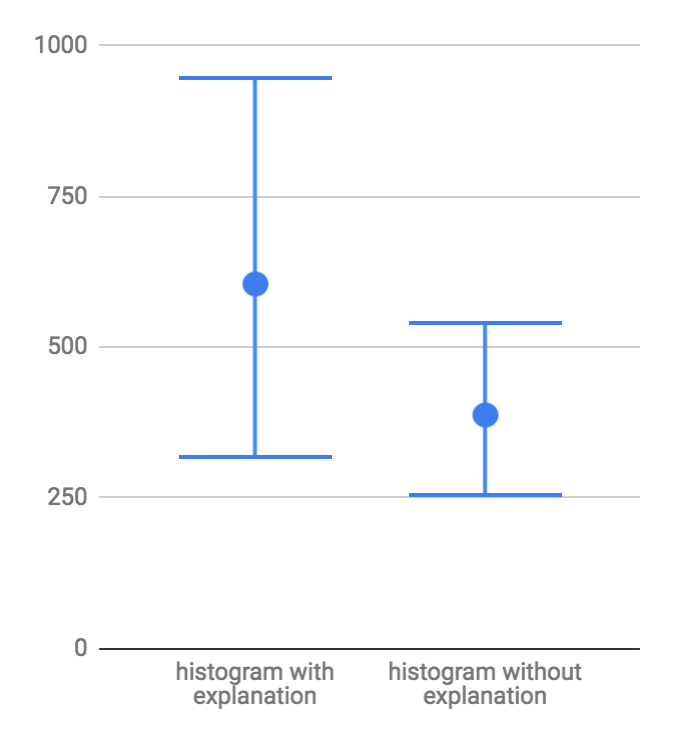
\includegraphics[width=0.4\linewidth]{figs/hist_interaction}
% \caption{
% Interaction with the histogram view measured by counting how many histogram bars were hovered by the mouse.
% The plot shows the bootstrapped mean and confidence interval for each setting.
% }
% \label{figs:hist_interaction}
% \end{figure}

Comparing the correctness across all four conditions can be seen in Figure~\ref{figs:correctness}.
First, we can see a strong improvement in correctness when adding explanations to histograms (p-value Fisher's $0.0359$, $\chi^2$ $0.0366$) or when switching from tables to histograms while having access to explanations (p-value Fisher's $0.0161$, $\chi^2$ $0.0169$).
We hypothesize that explanations are a necessity for histograms to work effectively, since they point out which, of the possibly many, pattern seen in the distributions are meaningful.
% The engagement with the histogram view was also higher when explanations were available (see Figure~\ref{figs:hist_interaction}).

\begin{figure}[b]
\centering
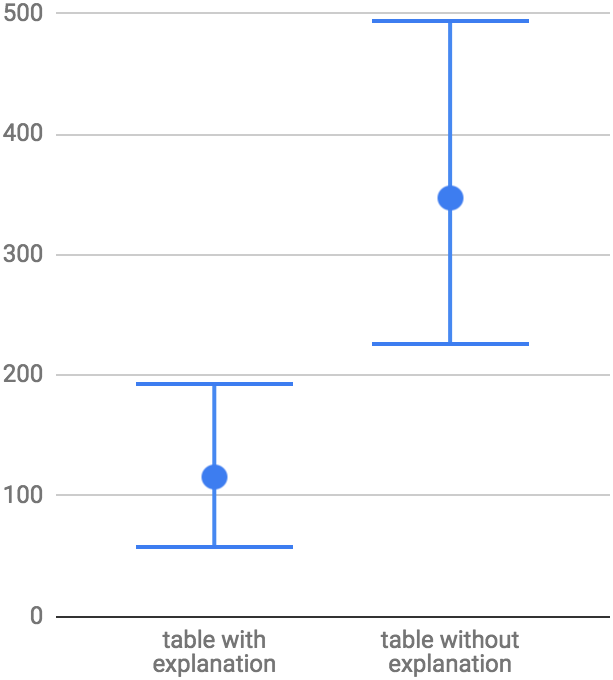
\includegraphics[width=0.4\linewidth]{aggexplain/table_interaction}
\caption{
Interaction with the table view measured by counting how many table cells were hovered by the mouse.
The plot shows the bootstrapped mean and confidence interval for each setting.
}
\label{figs:table_interaction}
\end{figure}

However, we see a strong decline in correctness when adding explanations to tables (p-value Fisher's $0.0311$, $\chi^2$ $0.0320$).
At first, we were puzzled at this counter-intuitive result and we double and triple checked that those results were not a simple mix-up in conditions.
We hypothesize that, having explanations at hand in a table, focuses the attention of participants to fewer instances and additionally makes them more confident that they fully understood the model.
This extrapolation from few instances aligns with the findings of Stumpf~\etal~\cite{harmful}, who found that explanations can be harmful in certain circumstances.

\begin{figure}[b]
\centering
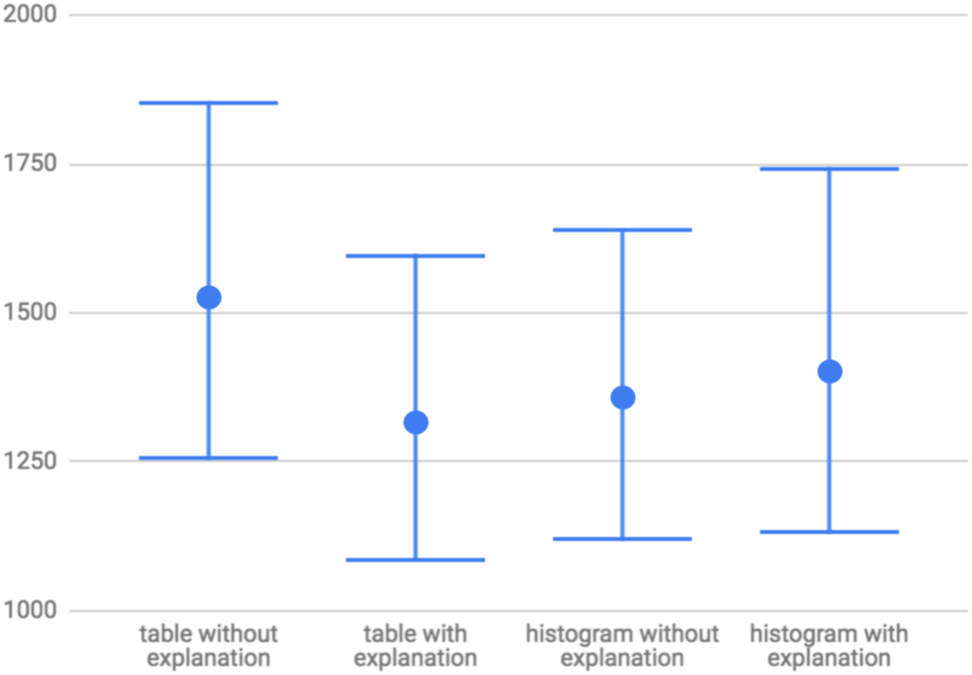
\includegraphics[width=0.6\linewidth]{aggexplain/timing2}
\caption{
Overall completion time of the study divided by condition.
The plot shows the bootstrapped mean and confidence interval for each setting.
There is no significant difference between the conditions.
}
\label{figs:timing}
\end{figure}

In order to investigate this hypothesis further, we can look at the number of interactions of the participants performing the tasks.
We can see in Figure~\ref{figs:table_interaction} that participants engaged with the table view significantly more when no explanations were present.
This might be an example of Hullman~\etal~\cite{6064986}, which states that information visualization might benefit from visual difficulties, as is the case with a table without any further help from the interface about what to look at, since people are forced to interact more with the visualization.

% \begin{figure*}
% \centering
% 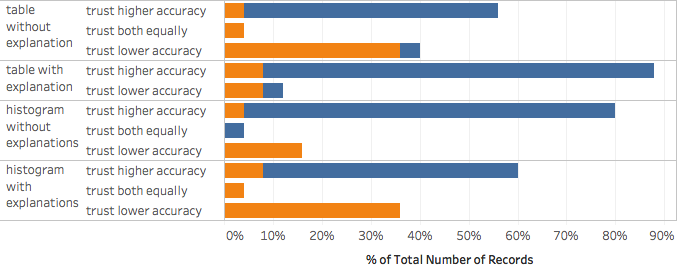
\includegraphics[width=0.75\linewidth]{figs/trust}
% \caption{
% The participants' answer to whether they trust the model with higher accuracy, lower accuracy, or both equally. The orange colored part indicates the proportion of participants that correctly found the bias in the data.
% Note, that some participants valued accuracy more than semantically correct data.
% }
% \label{figs:trust}
% \end{figure*}

Despite that, we found no significant difference in the time participants took to complete the study, as can be seen in Figure~\ref{figs:timing}.
% Additionally, Figure~\ref{figs:timing} also shows that participants spent less time on the histogram view with explanations than on the table view without explanations.
Even though the histogram view with explanations and the table view without explanations do not have a significant timing difference, we hypothesize that an aggregated representation of the model is a more effective method for finding biases.
This hypothesis is rooted in both conditions performing equally well and histograms being a more scalable data representation than tables, since due to their independence from the magnitude of the data.

As mentioned earlier, we chose the participants' written answers to determine whether the participant correctly identified the bias in the data.
Even though participants correctly identified the flaw in the data, it sometimes was not enough to convince them that the corresponding model cannot be trusted as much:
``If the data says it's true, then it's true I suppose and it's more trustworthy than my common sense.'';
``I feel like the results of [the biased model] where strange even though they where correct according to the dataset.'' (sic);
``I'm drawn to trusting the model which was more accurate even though it didn't entirely make sense to me.''.

$25\%$ of people who correctly identified the bias still opted to trust the biased model more, due to the higher reported accuracy of the model.
A further $8\%$ who identified the bias trusted both models equally.
Again, this aligns with the findings of Stumpf~\etal~\cite{harmful} that trust in the machine learning model may \emph{override} people's initial intuition about its performance.

% We categorized the written answers of the participants and noted when participants correctly detected the flaw in the biased data set (see Figure~\ref{figs:correctness}).
% Looking at the figure we can see a significant\todo{compute as well} improvement in correctly detected biases when changing either from the table view to the histogram view or from the having no explanations to having explanations.
% However, the condition of the table view without explanations has the highest rate of correct answers.
% Looking at the overall completion time (Figure~\ref{figs:timing}) we can see that participants without any help in form of aggregation or explanations spent more time analyzing the data set (Note, that the figure does not include extreme outliers at maximum 3 hours).
% This more thorough explanation enables the participants to find the bias in the data set even under non helpful conditions.
% In terms of trust (see Figure~\ref{figs:trust}) participants of the histogram view with explanations trust the correct model significantly\todo{compute} more than in the conditions with either only the histogram view or the table view with explanations.
% This is mostly in agreement with the ability to correctly identify the bias.
% However, some participants dismiss the unbiased model in favor of the higher accuracy of the biased model under all conditions: ``If the data says it's true, then it's true I suppose and it's more trustworthy than my common sense.''; ``I feel like the results of model 2 where strange even though they where correct according to the dataset.''; ``I'm drawn to trusting the model which was more accurate even though it didn't entirely make sense to me.''
% This might be partially rooted in the participants not feeling ``expert'' enough but stemmed mostly from regarding accuracy higher than the bias in the data.
% This aligns with the findings of Stumpf~\etal~\cite{harmful}.

\section{Discussion}
\label{sec:ag_discussion}
We showed that aggregating instance-level explanations can be an effective way of enabling humans to identify biases in the input data of machine learning tasks.
Even though, assisted aggregation is as effective as unassisted individual inspection it scales better with large data sets.
Individually inspecting instances in the data is only possible on a sample of the data and requires extrapolation of findings to the whole data set.
Aggregation does not suffer from this, as the representation of the data is independent from its size.
Even though, it requires dedication, our test data set was small enough to still be able to scan in full if necessary.

Furthermore, the bias planted in the data was simple enough to be able to be found in \emph{all} conditions.
This might not be true for real-world data sets with more complex biases.
Even though, histograms are advantageous with respect to tables in finding arbitrary patterns, they are still limited to only one dimension.
Biases that are present only through combinations of features will not be detectable.

In our study, we could confirm findings from Stumpf~\etal~\cite{harmful} and overcome their limitations by using instance-level explanations with aggregation.
However, we could not overcome trust in machine learning model authority, despite being confronted with contradictory evidence, in all cases.
Speculatively, this might stem from people being used to being presented with cleaned up and validated data, as this cumbersome process is often hidden from the end result.

% On this note, in order to guarantee that our data is of value, we experienced a high churn rate of eligible participants ($\geq1.16$ per eligible participant), even though the task seemed relatively simple, from the perspective of visual analytics researchers. \todo{meh, sounds braggy...} \todo{Do we even need to mention this?  I'd just remove.}

\section{Conclusion \& Future Work}
\label{sec:conclusion}
We presented a novel way of aggregating and comparing instance-level explanations.
We found that this method can help humans identify biases in the input data to machine learning models.
However, this is only the case in combination.
Aggregation alone or individual instance-level explanations might lead to worse performance in this regard.
We demonstrated, that an aggregated instance-level explanation approach is as effective as going through the data unassisted.
This is promising, as the proposed method is independent of the size of the data set and thus likely more scalable than its non-aggregated counterpart.
However, specifically confirming this hypothesis remains future work.

As we were conducting an exploratory analysis of the study, individual findings remain to be tested in-situ in future work.
Furthermore, experimenting with more complex forms of data biases opens up additional research opportunities.

All in all, we presented a usable method for effectively utilizing instance-level explanations on a large scale.
As machine learning models become more complex and opaque, this becomes an important stepping stone in tackling the behemoth of effectively improving machine learning models and their data alike.


%% if specified like this the section will be committed in review mode
% \acknowledgments{
% The authors wish to thank A, B, C. This work was supported in part by
% a grant from XYZ.}

% \bibliographystyle{abbrv}
%%use following if all content of bibtex file should be shown
%\nocite{*}
% \bibliography{template}
% \end{document}
